\chapter{Теоретическая часть}
\section{Содержательная и математическая постановки задачи о назаначениях}

\textbf{Содержательная постановка:} В распоряжении работодателя имеется $n$ работ и $n$ исполнителей. Стоимость выполнения $i\text{-ой}$ работы $j\text{-ым}$ исполнителем составляет $c_{ij} \geqslant 0$ единиц. Требуется распределить все работы между исполнителями так, чтобы:

\begin{enumerate}[label=\arabic*)]
    \item каждый исполнитель выполнял 1 работу;
    \item каждую работу выполнял только 1 исполнитель;
    \item общая стоимость выполнения всех работ была $\min$.
\end{enumerate}

Величины $c_{ij}$ принято записывать в матрицу:
$$
    C = (c_{ij}),\ i,j = \overline{1{,}n},
$$
которая называется матрицей стоимостей.

Введем управляемые переменные:
$$
    x_{ij} =
    \left.
    \begin{cases}
        1, & \text{если $i$-ую работу выполняет $j$-ый работник}, \\
        0, & \text{иначе},
    \end{cases}
    \right\},\ i, j = \overline{1{,}n}
$$

Управляемые переменные $x_{ij}$ записывают в матрицу
$$
    X = (x_{ij}),\ i,j = \overline{1{,}n},
$$
которая называется матрицей назначений. 

Тогда:
\begin{enumerate}[label=\arabic*)]
    \item Общая стоимость выполнения всех работ:
    $$
        f(x) = \sum\limits_{i=0}^n\sum\limits_{j=0}^nc_{ij}x_{ij}.
    $$
    \item Условие того что $\text{$i$-ую}$ работу выполняет один сотрудник:
    $$
        \sum\limits_{j=0}^nx_{ij} = 1,\ i = \overline{1{,}n}.
    $$
    \item Условие того что $\text{$j$-ый}$ работник выполняет ровно одну работу:
    $$
        \sum\limits_{i=0}^nx_{ij} = 1,\ j = \overline{1{,}n}.
    $$
\end{enumerate}

Таким образом приходим к \textbf{математической постановке} задачи о назначениях:

$$
\begin{cases}
    f = \sum\limits_{i=1}^n \sum\limits_{j=1}^n c_{ij} x_{ij} \rightarrow min, \\
    \sum\limits_{j=1}^n x_{ij} = 1, \: i = \overline{1{,}n}, \\
    \sum\limits_{i=1}^n x_{ij} = 1, \: j = \overline{1{,}n}, \\
    x_{ij} \in \{0, 1\}, \: i,j = \overline{1{,}n}.
\end{cases}
$$

\section{Краткое описание венгерского метода}

Схема венгерского метода решения задачи о назаначениях представлена на рисунках~\ref{fig:ven_meth_p}~---~\ref{fig:ven_meth_m}. 

\begin{figure}[H]
    \centering
    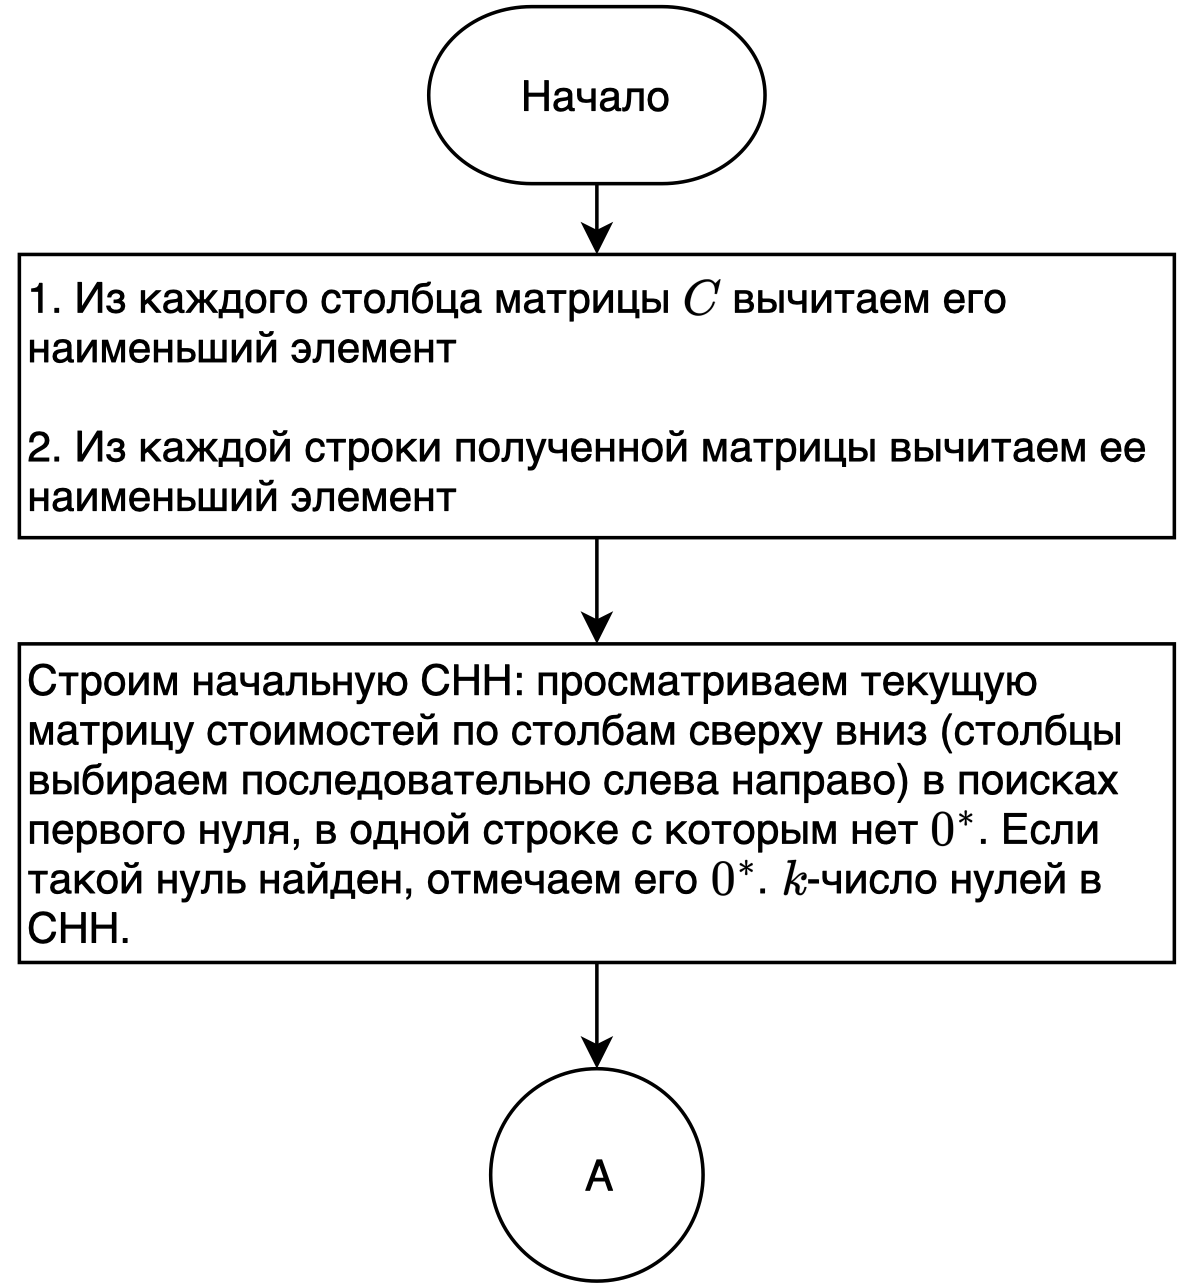
\includegraphics[width=0.4\linewidth]{./images/ven_meth_prep.png}
    \caption{Схема подготовительного этапа венгерского метода}
    \label{fig:ven_meth_p}
\end{figure}

\begin{figure}[h]
    \centering
    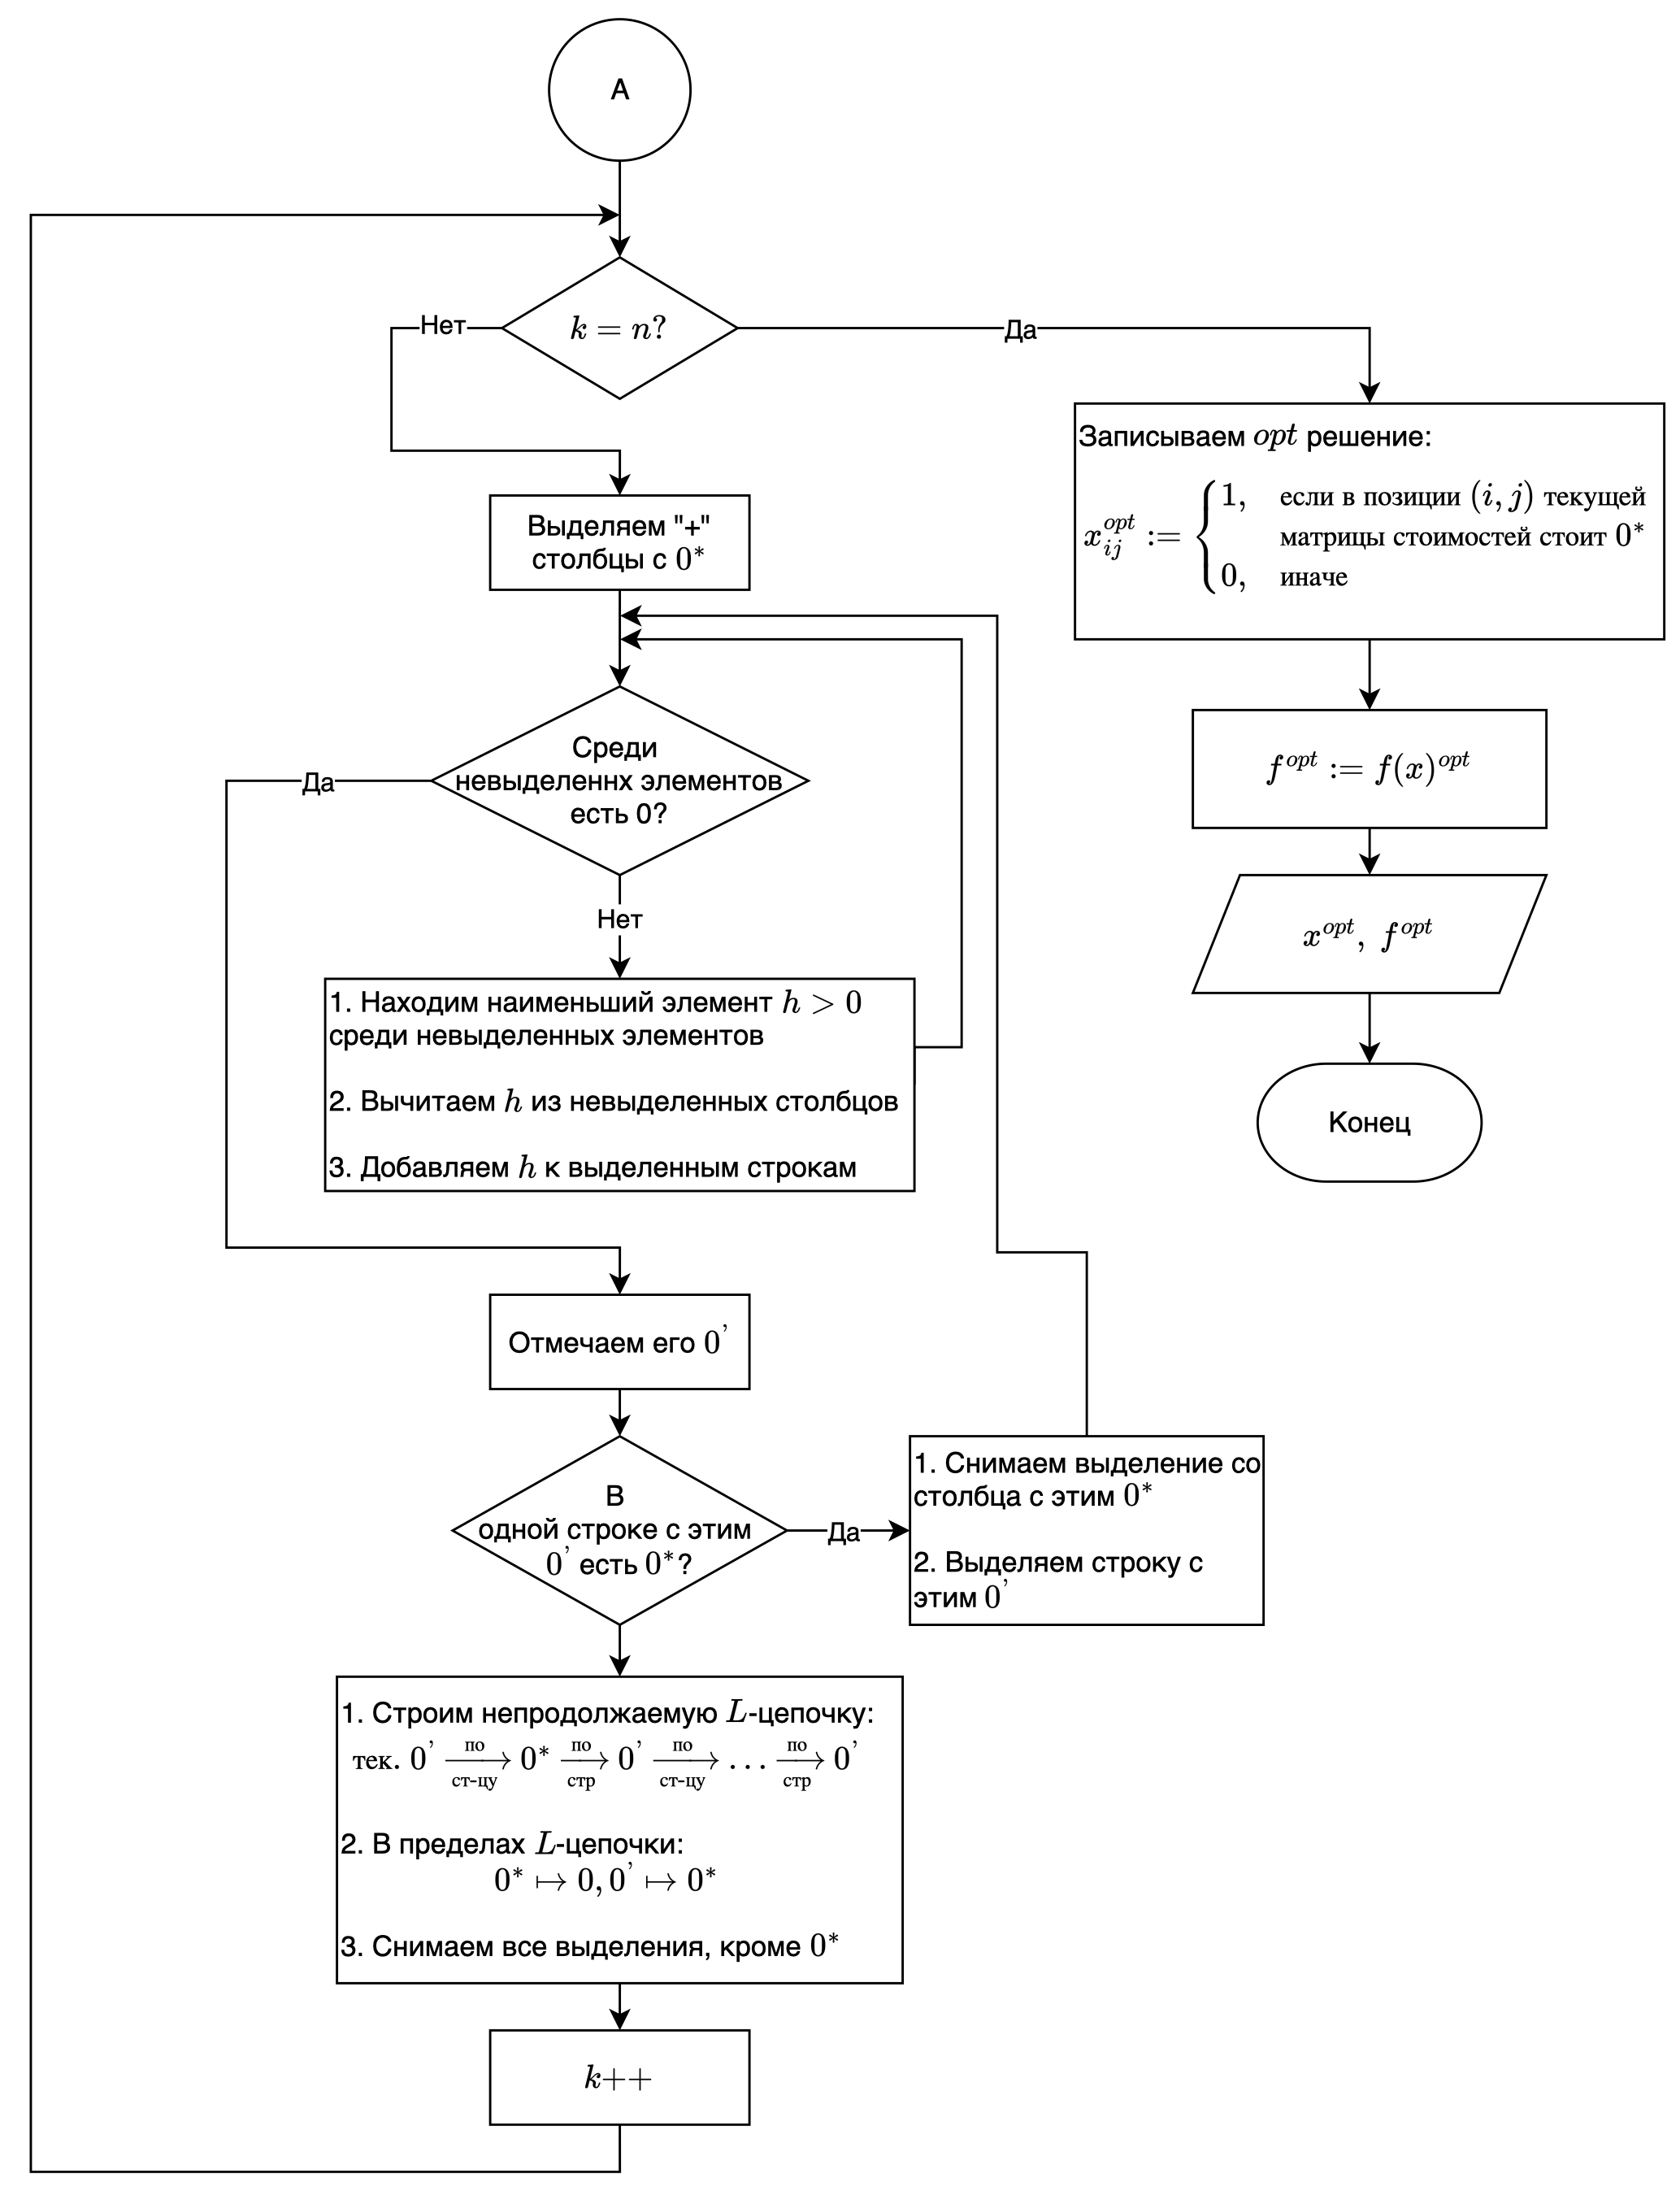
\includegraphics[width=0.9\linewidth]{./images/ven_meth_main.png}
    \caption{Схема основного этапа венгерского метода}
    \label{fig:ven_meth_m}
\end{figure}